\documentclass[a4paper,11pt]{article}

\usepackage[spanish]{babel}
\usepackage{multirow}
\usepackage{verbatim}
\usepackage{moreverb}
\usepackage{graphicx}

%Idioma
\usepackage[latin1]{inputenc}
%Letra arial
\usepackage{helvet}
%\renewcommand\familydefault{\sfdefault}
%Para incluir codigo fuente
\usepackage{listings}
%Para tener encabezados y pie de pagina personalizados
\usepackage{fancyhdr}
%Para poner eprafe en las imagenes
\usepackage[hang,bf]{caption2}


\usepackage{anysize}

%%------------Gráficos------------
%\%Paquete de gráficos
%\newif\ifpdf
%\ifx\pdfoutput\undefined
%	\pdffalse
%\else
%	\pdfoutput=1
%	\pdftrue
%\fi
%
%\ifpdf
%	\usepackage[pdftex]{graphicx}
%	\pdfcompresslevel=9
%\% 	\pdfcompresslevel=0
%	\usepackage{pdfpages}
%\else
%	\usepackage[dvips]{graphicx}
%\fi



% Titulo del Trabajo Practico.
\title{ Trabajo Pr\'actico 2: MIPS Datapath   \\
        \Large{ 66.20 Organizaci\'on de las Computadoras } }


% Informaci\'on sobre los autores.
\author{Nicol\'as Calvo, \textit{Padr\'on Nro. 78.914}           	\\
            \texttt{ nicolas.g.calvo@gmail.com }      			\\
            Celeste Maldonado, \textit{Padr\'on Nro. 85.630}              	\\
            \texttt{ maldonado.celeste@gmail.com }                             \\
            Matias Acosta, \textit{Padr\'on Nro. 88.590}                \\
            \texttt{ matiasja@gmail.com }                     		\\
            \LARGE{}         						\\
            \LARGE{}         						\\
            \LARGE{}         						\\
            \Large{2do. Cuatrimestre de 2011}         	\\                       
            \texttt{}         						\\
            \Large{Facultad de Ingenier\'\i{}a, Universidad de Buenos Aires}            \\
       }
\date{}



\begin{document}

\marginsize{2cm}{2cm}{2cm}{2cm}

\begin{figure}
\centering

\includegraphics[width=100pt]{logofiuba.jpg}
\end{figure}


\maketitle
\thispagestyle{empty}   % quita el numero en la primer pagina
%\renewcommand{\labelenumi}{\alph{enumi}.}


\newpage
% Declaro el indice

\tableofcontents
\newpage

\setcounter{page}{1}

\section{Introducci\'on}

\paragraph{}
En este trabajo, se busca el objetivo de familiarizarse con el camino de datos de la arquitectura MIPS y la implementaci\'on del pipeline de cinco etapas. 

\paragraph{}
Para la realizaci\'on del trabajo pr\'actico se implementaron segmentos de c\'odigo Assembly MIPS que fueron analizados posteriormente mediante a herramienta de simulaci\'on WinDLX .

\paragraph{}
La herramienta WinDLX permite simular una arquitectura MIPS 32 con pipeline de cinco etapas, pudiendo ver los valores de cada registro dentro del archivo de registros, la ejecuci\'on de instrucciones dentro de cada etapa del pipeline  y el acceso a estad\'isticas  de la ejecuci\'on, como la cantidad de ciclos que requiri\'o la ejecuci\'on o la cantidad y tipos de ciclos de stall.

\paragraph{}
Los resultados se analizaron con la opci\'on de forwarding activada y sin activar. 
Forwarding es la t\'ecnica utilizada para reducir la cantidad de ciclos de stall producidos ante un riesgo Read after Write (RAW), la cual consiste en adelantar el resultado de la etapa de ejecuci\'on de la instrucci\'on que escribe el registro a ser le\'ido en una instrucci\'on pr\'oxima, de manera que las instrucciones siguientes que requieran del contenido actualizado de dicho registro puedan acceder al mismo antes de haber sido escrito en la etapa de Write-Back.

\newpage 

\section{Desarrollo}

\begin{enumerate}

% PUNTO 1
\item  Realizar las siguientes operaciones:

\begin{center}
\begin{verbatim}
A=4
B=5
C=7
D=3
X=B+C
Y=D-C
Z=(((((A+C)-B)*C)-X)/Y)
A=X*Y*3
\end{verbatim}
\end{center}

Donde las variables A,B,C,D est\'an en memoria. La variable Z es de tipo double. Determinar el CPI para el conjunto de las operaciones, cantidad y tipo de Stalls.

\paragraph{}
\underline{\textsc{Resoluci\'on:}}

\paragraph{Ejecuci\'on del programa sin forwarding}


\paragraph{}
Se ejecutan X ciclos y X instrucciones , con 2 instrucciones en el  pipeline al finalizar.

\paragraph{}
\begin{center}
$CPI = X  ciclos /x instrucciones = x$
\end{center}

\paragraph{}

Se contaron un total de X stalls, divididos en las siguientes categor\'ias:

\begin{itemize}
\item x stalls de control (x\% de todos los ciclos)
\item x  stalls correspondientes a la instruccion trap (x\% de todos los ciclos)
\item x stalls RAW (Read After Write) (x\% de todos los ciclos).
\end{itemize}

\paragraph{Ejecuci\'on del programa con forwarding:}


\paragraph{}
Se ejecutan X ciclos y X instrucciones , con x instrucciones en el  pipeline al finalizar.

\paragraph{}
\begin{center}
$CPI = x ciclos / x  instrucciones = x$
\end{center}

\paragraph{} 

Se contaron un total de x stalls, divididos en las siguientes categor\'ias:

\begin{itemize}
\item x stalls de control (x\% de todos los ciclos)
\item x stalls correspondientes a la instruccion trap (x\% de todos los ciclos)
\item x stalls RAW (Read After Write) (x\% de todos los ciclos).
\end{itemize}


\newpage

% PUNTO 2
\item	Realizar un reordenamiento del c\'odigo assembly implementado en el \'item anterior que disminuya el CPI.

\paragraph{}
\underline{\textsc{Resoluci\'on:}}

Se reorden\'o el codigo moviendo a la instrucci\'on 

\begin{verbatim}
%andi r3,r2,#1 
\end{verbatim}


de la siguiente forma:

\paragraph{}
Codigo original:

\begin{center}
\begin{verbatim}
	sge r8,r2,r5
	bnez r8,Fin 
	andi r3,r2,#1 
	bnez r3,Modulo 
	add r1,r1,r2
\end{verbatim}
\end{center}

\paragraph{} 
Codigo reordenado:

\begin{center}
\begin{verbatim}
	sge r8,r2,r5 
	andi r3,r2,#1 
	bnez r8,Fin 	 
	bnez r3,Modulo 
	add r1,r1,r2
\end{verbatim}
\end{center}

\paragraph{}
Se obtuvieron los siguientes resultados:

\paragraph{Ejecucion sin forwarding:}

\paragraph{}
Se ejecutan x ciclos y x instrucciones , con x instrucciones en el  pipeline al finalizar.

\begin{center}
$CPI = x ciclos / x instrucciones = x $
\end{center}

\paragraph{}

Se contaron un total de x stalls, divididos en las siguientes categor\'ias:

\begin{itemize}
 \item x stalls de control (x\% de todos los ciclos)
 \item  x  stalls correspondientes a la instruccion trap (x\% de todos los ciclos)
 \item  x stalls RAW (Read After Write) (x\% de todos los ciclos)
\end{itemize}

\paragraph{Ejecuci\'on con forwarding:}

\paragraph{}
Se ejecutan x ciclos y x instrucciones , con x instrucciones en el  pipeline al finalizar.

\begin{center}
$CPI = x ciclos / x instrucciones = x$
\end{center}


\paragraph{} 
Se contaron un total de x stalls, divididos en las siguientes categor\'ias:

\begin{itemize}
 \item x stalls de control (x\% de todos los ciclos)
 \item x stalls correspondientes a la instruccion trap (x\% de todos los ciclos)
 \item x  stalls RAW (Read After Write) (x\% de todos los ciclos)
\end{itemize}


\newpage
% PUNTO 3
\item Implementar el siguiente segmento de c\'odigo en Assembly MIPS:


\lstset{language=c,basicstyle=\small,showstringspaces=false,columns=fullflexible,frame=lines,tabsize=4,inputencoding=latin1,extendedchars=true}
\lstinputlisting{E3_codigoc.c}

Determinar el CPI para el conjunto de las operaciones, cantidad y tipo de Stalls. Verificar la posibilidad de utilizar branch delay slot para realizar una mejora en el tiempo de ejecuci\'on.

\paragraph{}
\underline{\textsc{Resoluci\'on:}}


\paragraph{Ejecuci\'on del programa sin forwarding}


\paragraph{}
Se ejecutan 129 ciclos y 64 instrucciones , con 2 instrucciones en el  pipeline al finalizar.

\paragraph{}
\begin{center}
$CPI = 129 ciclos / 64 instrucciones = 2.02$
\end{center}

\paragraph{}

Se contaron un total de 64 stalls, divididos en las siguientes categor\'ias:

\begin{itemize}
\item 10 stalls de control (7.75\% de todos los ciclos)
\item 2  stalls correspondientes a la instruccion trap (1.55\% de todos los ciclos)
\item 52 stalls RAW (Read After Write) (40.31\% de todos los ciclos).
\end{itemize}

\paragraph{Ejecuci\'on del programa con forwarding:}


\paragraph{}
Se ejecutan 98 ciclos y 64 instrucciones , con 2 instrucciones en el  pipeline al finalizar.

\paragraph{}
\begin{center}
$CPI = 98 ciclos / 64 instrucciones = 1,53$
\end{center}

\paragraph{}
Se logr\'o un $SpeedUp = 1.32$

\paragraph{} 

Se contaron un total de 33 stalls, divididos en las siguientes categor\'ias:

\begin{itemize}
\item 10 stalls de control (10.20\% de todos los ciclos)
\item 2  stalls correspondientes a la instruccion trap (2.04\% de todos los ciclos)
\item 21 stalls RAW (Read After Write) (21.43\% de todos los ciclos), de los cuales los 21 corresponden a stalls de branch, es decir, que dichos branches tienen por argumentos registros escritos en la instruccion que los precede.
\end{itemize}

\paragraph{} 
Para el codigo presentado Branch Delay Slot no podría usarse para lograr una mejora significativa en tiempo de ejecuci\'on debido a las dependencias de los branches respecto a los argumentos de las instrucciones que se ejecutan antes y despues de ellos.


\paragraph{} 
Por ejemplo, para el segmento:

\begin{center}
\begin{verbatim}
		andi r3,r2,#1 
		bnez r3,Modulo 
		add r1,r1,r2 
Modulo:	sgt r8,r1,r6
\end{verbatim}
\end{center}

\paragraph{} 

La instruccion andi se usa en el branch, por lo que no puede moverse al delay slot y sgt requiere de un registro que es modificado en caso de no tomar el branch, por lo que mover esta instruccion al delay slot modificar\'ia la logica del programa.

\newpage

% PUNTO 4
\item

Realizar un reordenamiento del c\'odigo assembly implementado en el \'item anterior que disminuya el CPI.

\paragraph{}
\underline{\textsc{Resoluci\'on:}}

\paragraph{} 
Se reorden\'o el codigo moviendo a la instrucci\'on 

\begin{verbatim}
andi r3,r2,#1 
\end{verbatim}


de la siguiente forma:

\paragraph{}
Codigo original:

\begin{center}
\begin{verbatim}
	sge r8,r2,r5
	bnez r8,Fin 
	andi r3,r2,#1 
	bnez r3,Modulo 
	add r1,r1,r2
\end{verbatim}
\end{center}

\paragraph{} 
Codigo reordenado:

\begin{center}
\begin{verbatim}
	sge r8,r2,r5 
	andi r3,r2,#1 
	bnez r8,Fin 	 
	bnez r3,Modulo 
	add r1,r1,r2
\end{verbatim}
\end{center}

\paragraph{}

De esta forma se espera reducir los ciclos de stall RAW para que bnez r3, Modulo tenga disponible el valor del registro r3. Algo similar suceder\'ia para bnez r8,Fin respecto a sge r8,r2,r5.

\paragraph{}
Se obtuvieron los siguientes resultados:

\paragraph{Ejecucion sin forwarding:}

\paragraph{}
Se ejecutan 108 ciclos y 64 instrucciones , con 2 instrucciones en el  pipeline al finalizar.

\begin{center}
$CPI = 108 ciclos / 64 instrucciones = 1.69 $
\end{center}

\paragraph{}

Se contaron un total de 43 stalls, divididos en las siguientes categor\'ias:

\begin{itemize}
 \item 10 stalls de control (9.26\% de todos los ciclos)
 \item  2  stalls correspondientes a la instruccion trap (1.85\% de todos los ciclos)
 \item  31 stalls RAW (Read After Write) (28.70\% de todos los ciclos)
\end{itemize}

\paragraph{}
SpeedUp respecto al codigo $sin reordenamiento = 1.2$

\paragraph{Ejecuci\'on con forwarding:}

\paragraph{}9
Se ejecutan 84 ciclos y 64 instrucciones , con 2 instrucciones en el  pipeline al finalizar.

\begin{center}
$CPI = 84 ciclos / 64 instrucciones = 1.31$
\end{center}

\paragraph{}
SpeedUp respecto al codigo$ sin reordenamiento = 1.17$

\paragraph{} 

Se contaron un total de 19 stalls, divididos en las siguientes categor\'ias:

\begin{itemize}
 \item 10 stalls de control (11.09\% de todos los ciclos)
 \item  stalls correspondientes a la instruccion trap (2.38\% de todos los ciclos)
 \item stalls RAW (Read After Write) (8.33\% de todos los ciclos), de los cuales los 7 corresponden a stalls de branch, es decir, que dichos branches tienen por argumentos registros escritos en la instruccion que los precede.
\end{itemize}

\newpage

% PUNTO 5
\item Implementar un segmento de c\'odigo que con la adici\'on de instrucciones de tipo nop mejore su desempeno. Si no fuera posible, explicar los motivos.

\underline{\textsc{Resoluci\'on:}}

\paragraph{Riesgos Estructurales}

\paragraph{}
Los riesgos reducen el rendimiento de la velocidad ideal lograda por la segmentaci\'on. Hay tres clases de riesgos:
\paragraph{}
1. Riesgos estructurales surgen de conflictos de los recursos, cuando el hardware no puede soportar todas las combinaciones posibles de instrucciones en ejecuciones solapadas simult\'aneamente.
\paragraph{}
2. Riesgos por dependencias de datos surgen cuando una instrucci\'on depende de los resultados de una instrucci\'on anterior, de forma que, ambas, podr\'ian llegar a ejecutarse de forma solapada.
\paragraph{}
3. Riesgos de control surgen de la segmentaci\'on de los saltos y otras instrucciones que cambian el PC.

\paragraph{}
Riesgos por dependencias de datos:
\paragraph{}
El problema de la dependencia de datos entre una instrucci\'on I1 y otra I2 que sigue, puede prevenirse retrasando la ejecuci\'on de I2 un n\'umero de K de etapas hasta que desaparezca el problema de que I2 lea un operando que I1 no ha escrito todav\'ia. 
\paragraph{}
Este retraso puede conseguirse insertando un n\'umero K de instrucciones entre I1 e I2. Esto significa que el compilador tiene que reordenar el programa para encontrar K instrucciones que puedan ejecutarse despu\'es de I1 y antes de I2 sin que ello var\'ie la estructura l\'ogica del problema.
\paragraph{}
Si el compilador no puede reorganizar el c\'odigo para encontrar esas K instrucciones antes mencionadas, sin modificar la l\'ogica del programa, debe insertar operaciones NOP (no operaci\'on) entre I1 e I2.

\paragraph{}
Si se trata de una instrucci\'on de salto, hasta que no llega a la etapa de ejecuci\'on no se establece en el PC la direcci\'on de la siguiente instrucci\'on a ejecutar, por lo que la etapa alimentaci\'on de instrucci\'on no sabe por donde seguir alimentando instrucciones. La etapa de alimentaci\'on no puede extraer la siguiente instrucci\'on a una bifurcaci\'on hasta que esta \'ultima no finalice su etapa de ejecuci\'on, \'esta tendr\'ia que esperar hasta que se alimente la siguiente instrucci\'on y vaya avanzando por todos las etapas anteriores, que se habr\'an quedado vac\'ias. A estas etapas vac\'ias se las llama huecos de retardo (delay slots).
\paragraph{}
Nos encontramos con la misma soluci\'on, en la cual debemos reorganizar el c\'odigo para rellenar los huecos de retardo con instrucciones \'utiles.
Si no es posible reordenar el c\'odigo sin afectar la sem\'antica, se debe insertar operaciones NOP en los huecos de retardo.

\paragraph{}
A continuaci\'on mostraremos un segmento de c\'odigo con riesgo RAW:


\begin{center}
\begin{verbatim}
main:
                add             r1,r2,r3
                lw              r4,0(r1)        ;load into r4 using r1
                sw              12(r1),r4       ;store r4 using r1
                lw              r1,0(r2)
                sub             r4,r1,r5
                and             r6,r1,r7
                or              r8,r1,r9
Finish:       
                trap            0
\end{verbatim}
\end{center}

\paragraph{}
\centering
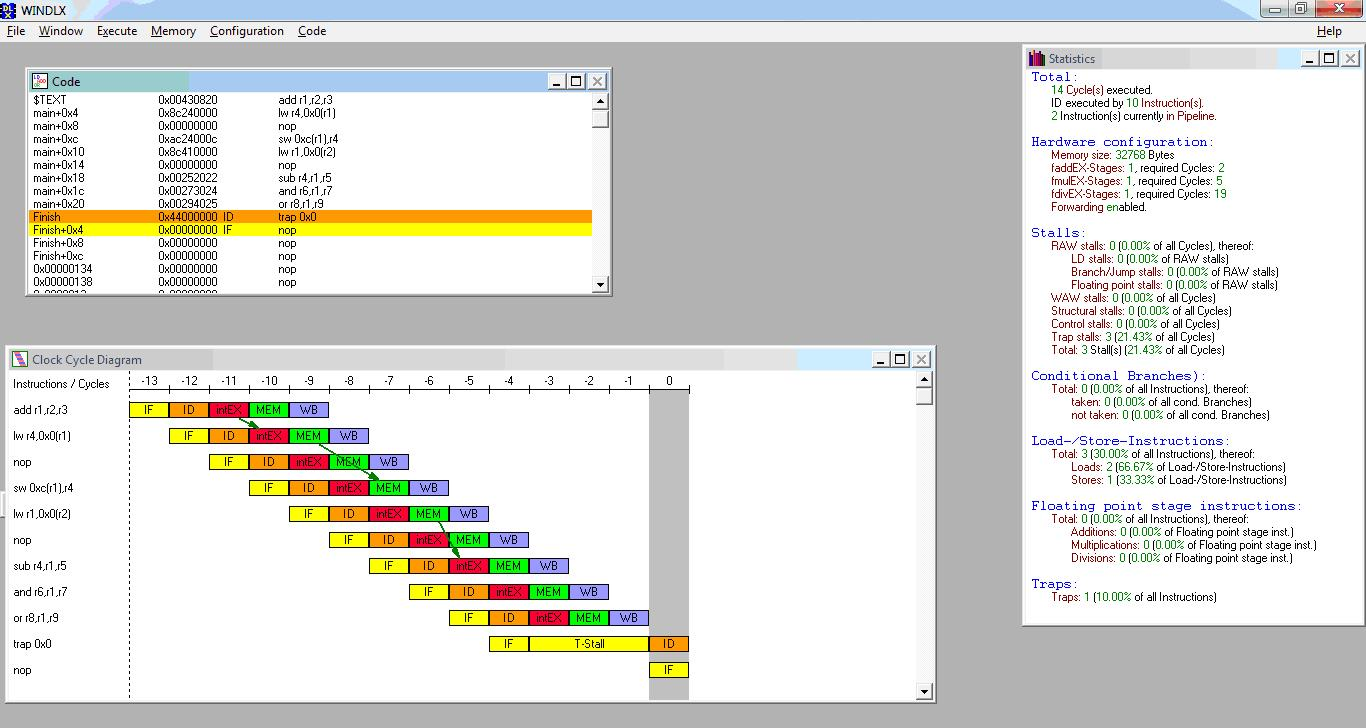
\includegraphics[width=400pt]{punto5-1.JPG}


\paragraph{}
Ahora, utilizaremos nop para evitar los riesgos producidos.
\begin{center}
\begin{verbatim}
main:
                add             r1,r2,r3
                lw              r4,0(r1)        ;load into r4 using r1
				nop
                sw              12(r1),r4       ;store r4 using r1
                lw              r1,0(r2)
				nop
                sub             r4,r1,r5
                and             r6,r1,r7
                or              r8,r1,r9
Finish:       
                trap            0
\end{verbatim}
\end{center}

\paragraph{}
\centering
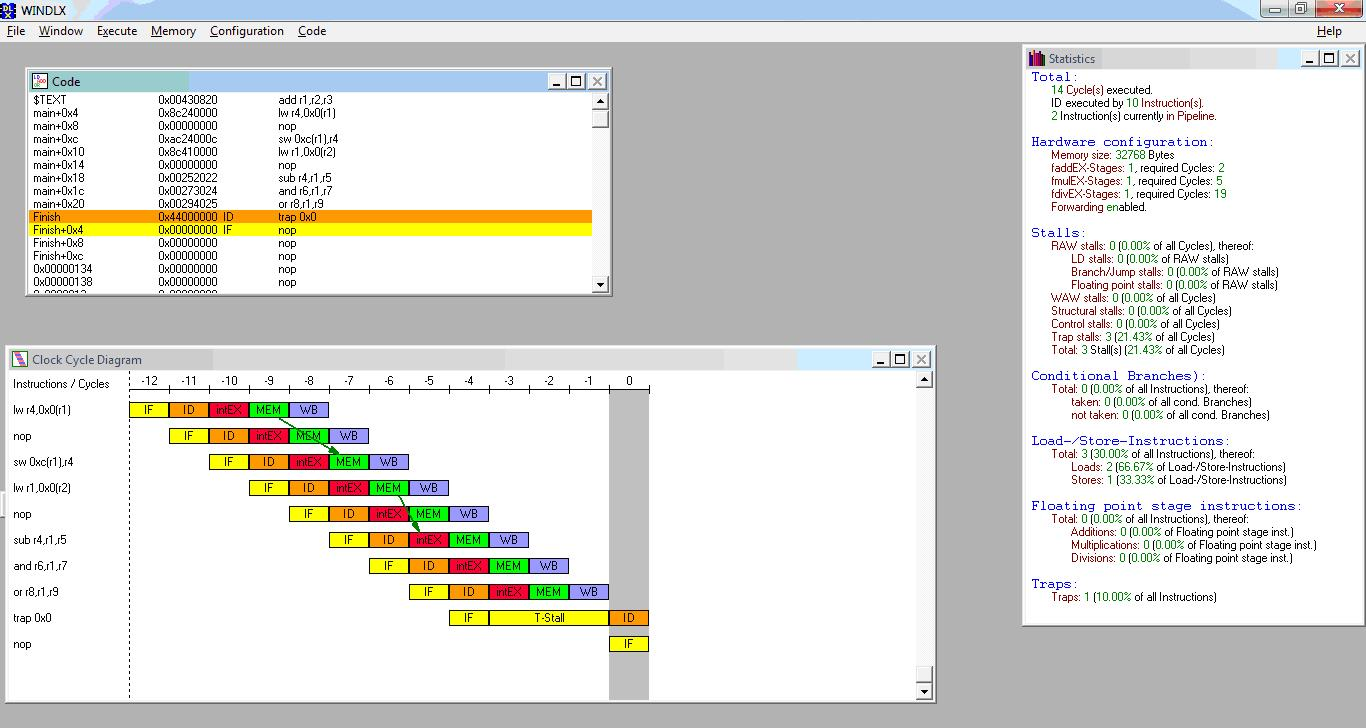
\includegraphics[width=400pt]{punto5-2.JPG}

\paragraph{}
Como se puede apreciar, no hay beneficio en cuanto a la cantidad de ciclos necesarios para ejecutar el programa.

\paragraph{}
Ahora veremos un riesgo por salto condicional.

\begin{center}
\begin{verbatim}
		.data 0
dato: 	.word 1
		.text
main:
		addi r20, r0, dato
		addi r30, r0, 20
		xor r1, r1, r1
loop: 	xor r2, r2, r2
		and r3, r4, r5
		subui r30, r30, 1
		add r6, r7, r8
		add r9, r10, r11
		addui r1, r1, 1
		bnez r30, loop
		trap #0
\end{verbatim}
\end{center}

\paragraph{}
\centering
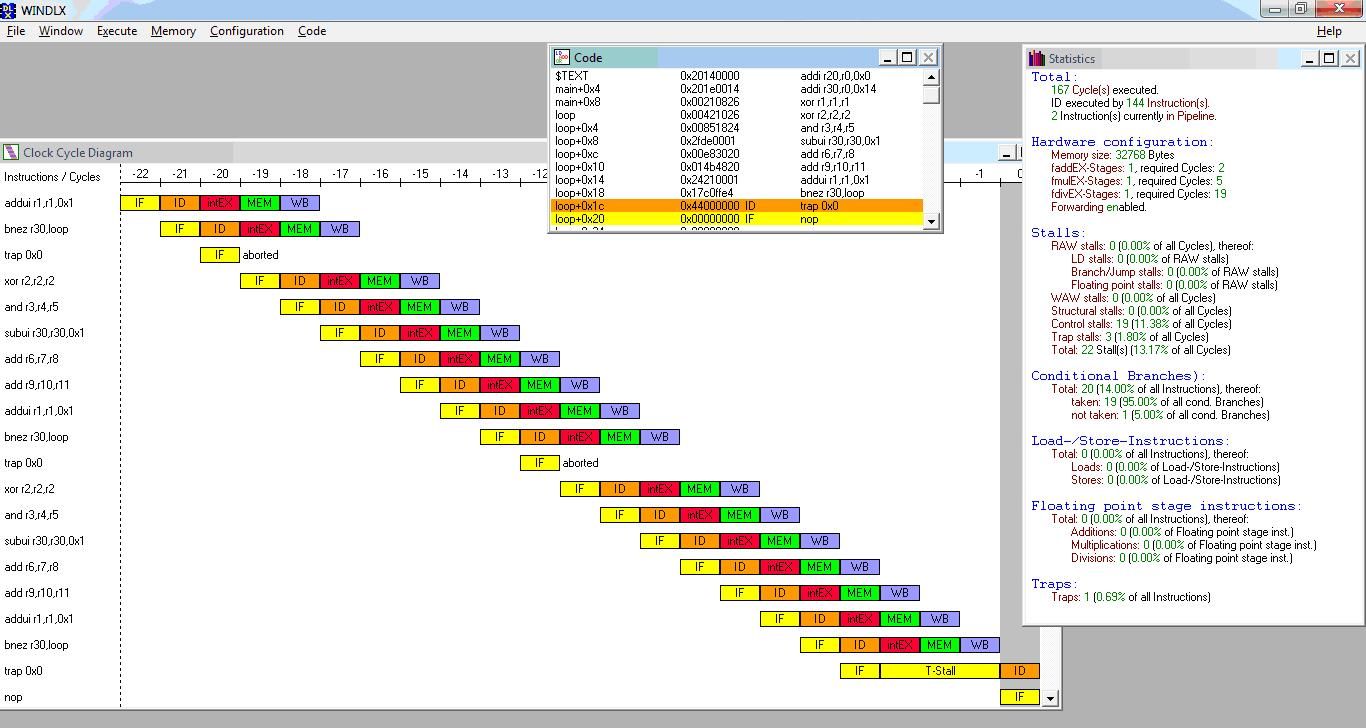
\includegraphics[width=400pt]{punto5-3.JPG}

\paragraph{}
\begin{center}
\begin{verbatim}
Ahora utilizando nop:

		.data 0
dato: 	.word 1
		.text
main:
		addi r20, r0, dato
		addi r30, r0, 20
		xor r1, r1, r1
loop: 	xor r2, r2, r2
		and r3, r4, r5
		subui r30, r30, 1
		add r6, r7, r8
		add r9, r10, r11
		addui r1, r1, 1
		bnez r30, loop
		nop
		trap #0
\end{verbatim}
\end{center}

\paragraph{}
\centering
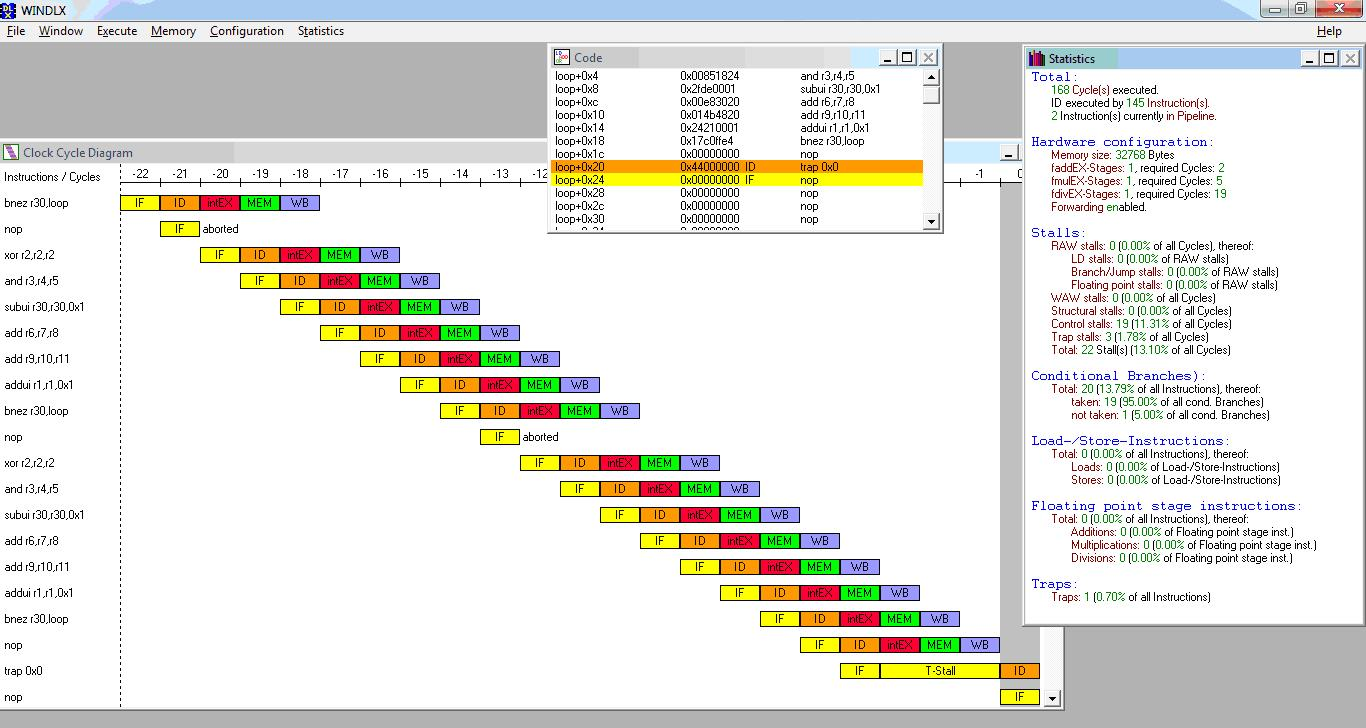
\includegraphics[width=400pt]{punto5-4.JPG}

\paragraph{}
Se puede ver que el segmento de c\'odigo se ha ejecutado en 168 ciclos, uno m\'as que sin utilizar el comando NOP.



\end{enumerate}

\newpage 

\section{Conclusi\'on}
\paragraph{}
Como conclusi\'on, podemos decir que el comando NOP, solo sirve para evitar riesgos pero no para acelerar el procesamiento del c\'odigo.



\end{document}

